\documentclass{beamer}
\usepackage[T1]{fontenc}
\usepackage{mathtools}
\usepackage{hyperref}
\usepackage{graphicx}
\usepackage{amsmath}
\usepackage{multicol}
\usepackage[export]{adjustbox}
\usepackage{scalerel}

\DeclarePairedDelimiter\floor{\lfloor}{\rfloor}
\DeclarePairedDelimiter\bra{\langle}{\rvert} 
\DeclarePairedDelimiter\ket{\lvert}{\rangle}
\DeclarePairedDelimiterX\braket[2]{\langle}{\rangle}{#1 \delimsize\vert #2}

\title{Modele obliczeń kwantowych}
\author{Jakub Zieliński}
\institute{Wydział Elektroniki i Technik Informacyjnych\\ Politechnika Warszawska}
\date{}
\usetheme{Warsaw}


\newcommand{\tens}[1]{%
	\mathbin{\mathop{\otimes}\displaylimits_{#1}}%
}
\begin{document}
	
	
	\begin{frame}
	\titlepage
	\end{frame}
	
	\begin{frame}{Aparat matematyczny}
		
		\begin{block}{Notacja Diraca, "bra-ket"}
			\vspace{0.5em}
			Używana do opisu wektorów z tzw. przestrzeni Hilberta ($\bra{bra}$ jest hermitowskim sprzężeniem $\ket{ket}$).\\~\\
			Jeżeli $\ket{ket}$ jest wektorem kolumnowym \\~\\
			\centering
			$
			\begin{pmatrix}
			\alpha_{1} &\alpha_{2} & \cdots &\alpha_{n-1} &\alpha_{n} 
			\end{pmatrix}
			^{T}
			$\\~\\
			\flushleft
			to $\bra{bra}$ jest wektorem w postaci rzędu\\~\\ 
			\centering
			$
			\begin{pmatrix}
			\beta_{1} &\beta_{2} & \cdots &\beta_{n-1} &\beta_{n} 
			\end{pmatrix}
			$
			\vspace{0.5em}
		\end{block}
	\end{frame}	

	\begin{frame}{Aparat matematyczny}
		\begin{block}{Podstawowe opercje}
			\vspace{0.5em}
			\begin{enumerate}
				\item iloczyn skalarny $\braket{bra}{ket}$
				\item rzutowanie na wektor $\ket{v_{1}}\braket{v_{1}}{v_{2}}$ (rzut $v_{2}$ na $v_{1}$)
				\item zapis wektora w bazie $$\ket{V} = \sum\limits_{i=1}^n \alpha_{i}\ket{v_{i}}$$
			\end{enumerate}	
			\vspace{0.5em}
		\end{block}
	\end{frame}
	
	\begin{frame}
		\begin{block}{Przykład nr 1 - Rozkład w bazie}
			\vspace{0.5em}
			Wektor w bazie o wymiarze $n=3$ możemy zapisać w następujący sposób:
				\begin{equation*}
					\ket{\psi} = \alpha\ket{001} + \beta\ket{010} + \gamma\ket{100}
				\end{equation*}
			$\ket{001},\ket{010},\ket{100}$ są wyłącznie etykietami.
			
			\vspace{0.5em}
		\end{block}
	
		\begin{block}{Przykład nr 2 - Rzutowanie}
			\vspace{0.5em}
			Weźmy wektor  $\ket{V} = \sum\limits_{i=1}^n \alpha_{i}\ket{v_{i}}$.\\~\\
			Rzutujmy wektor $\ket{V}$ na ortonormalny wektor bazowy $\ket{v_{1}}$.\\~\\
			$\ket{v_{1}}\bra{v_{1}}\ket{V}=
			\alpha_{1}\ket{v_{1}}\overbrace{\braket{v_{1}}{v_{1}}}^{1} +
			 \alpha_{2}\ket{v_{1}}\overbrace{\braket{v_{1}}{v_{2}}}^{0} +...+
			 \alpha_{n}\ket{v_{1}}\overbrace{\braket{v_{1}}{v_{n}}}^{0} 
			$\\~\\
			Otrzymujemy $\ket{v_{1}}\bra{v_{1}}\ket{V}= \alpha_{1}\ket{v_{1}}\braket{v_{1}}{v_{1}}=\alpha_{1}\ket{v_{1}}$
			
			\vspace{0.5em}
		\end{block}
	\end{frame}
			
	\begin{frame}{Czym jest kubit?}
		
		\begin{block}{Opis matematyczny}
		\vspace{0.5em}
		Układ opisany dwuwymiarową przestrzenią Hilberta. Kubit jest superpozycją 2 podstawowych stanów własnych $\ket{0}$ i $\ket{1}$.\\
		\begin{equation*}
			\ket{\psi_{0}} = \alpha\ket{0} + \beta\ket{1}
		\end{equation*}
		Gdzie $\alpha^{2}$ i $\beta^{2}$ są prawdopodobieństwami wystąpienia odpowiednich stanów własnych oraz $$\lVert\alpha\rVert^{2} + \lVert\beta\rVert^{2} = 1$$
		
		\vspace{0.5em}
		\end{block}			
	\end{frame}

	
	\begin{frame}{}
		\begin{block}{Sfera Blocha}
			\vspace{0.5em}
			Kubit może być również przy pomocy funkcji trygonometrycznych.
			\begin{equation*}
			\ket{\psi_{0}} = \cos{\frac{\theta}{2}}\ket{0} + e^{i\phi}\sin{\frac{\theta}{2}}\ket{1} 
			\end{equation*}
			gdzie $0\leq\phi\leq\pi$ i $0\leq\theta\leq2\pi$\\~\\
			Pozwala to na przedstawienie kubitu jako sfery Blocha.
			\vspace{0.5em}
		\end{block}
		\begin{figure}[hbt!]
			\centering
			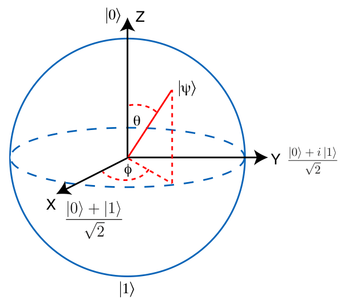
\includegraphics[scale=0.8]{media/bloch.png}
		\end{figure}		
	\end{frame}

	\begin{frame}{Pomiar stanu kubitu}
		\begin{block}{}
			\vspace{0.5em}
			Na wynik pomiaru stanu kubitu wpływa jego opis w przestrzeni Hilberta, tzn. wartości współczynników $\alpha$ i $\beta$.
			Co więcej, pomiar powoduje zmianę stanu układu. Następuje $\href{https://en.wikipedia.org/wiki/Wave_function_collapse}{collapse}$ i stan układu przyjmuj wartość pomiaru. $np. \ket{\phi} \longrightarrow \ket{1}$
			\vspace{0.5em}
		\end{block}
		
		\vspace{0.5em}
		\begin{center}
			\begin{figure}
				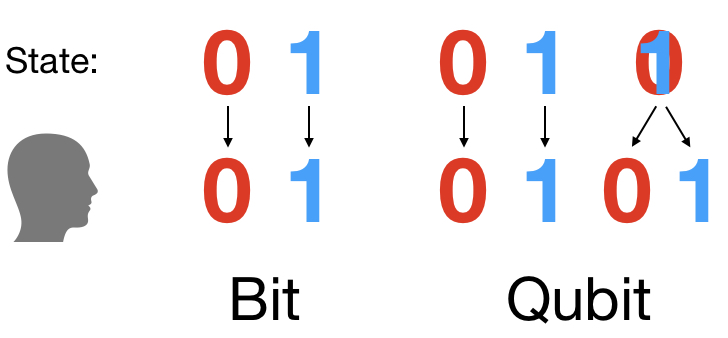
\includegraphics[scale=0.25]{media/collapse.jpg}
			\end{figure}
		\end{center}
		\vspace{0.5em}
	\end{frame}

	\begin{frame}{Pomiar stanu kubitu}
			\begin{block}{}
			\vspace{0.5em}
			Jeżeli jako fizyczny model naszego kubitu uznamy foton, to pomiar stanu możemy sobie wyobrazić jako przepuszczenie przez polaryzator.
			\vspace{0.5em}
		\end{block}
	
		\begin{figure}
			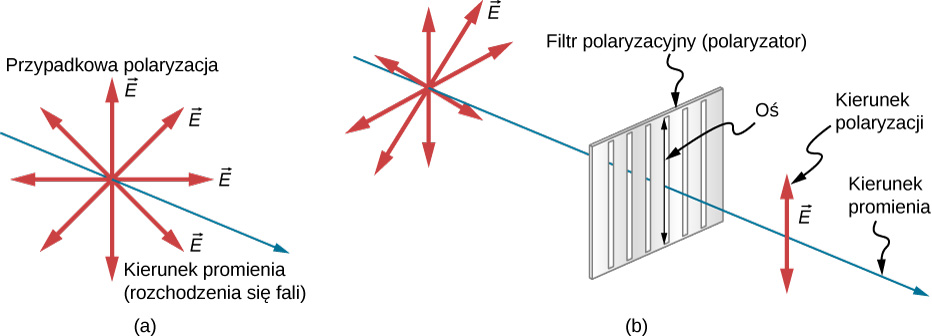
\includegraphics[scale=0.33]{media/foton_pomiar.png}
		\end{figure}
	\end{frame}
	
	\begin{frame}{Podstawowe operacje na kubitach}
		\begin{block}{   }
			\vspace{0.5em}
			Zdefiniujmy wektory własne $\ket{0}$ i $\ket{1}$ odpowiednio jako
			$\begin{pmatrix}
				1\\
				0
			\end{pmatrix}$
			i
			$\begin{pmatrix}
				0\\
				1
			\end{pmatrix}$
			\\~\\
			Łatwo sprawdzić, że wektory są ortonormalne, czyli
			\begin{multicols}{4}
				$\braket{0}{0} = 1$\\
				$\braket{1}{1} = 1$\\
				$\braket{1}{0} = 0$\\
				$\braket{0}{1} = 0$
			\end{multicols}
			\vspace{0.5em}
		\end{block}
	
		\begin{center}
			\begin{figure}
				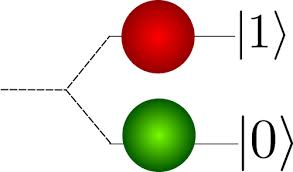
\includegraphics[scale=0.53]{media/qubits.jpeg}
			\end{figure}
		\end{center}
	\end{frame}

	\begin{frame}{Bramki kwantowe}
		\begin{block}{Bramka Hadamarda}
			\vspace{0.5em}
			Jedno-kubitowa bramka oznaczana $\hat{H}$, opisana macierzą\\
				
			\begin{columns}
				\begin{column}{0.33\textwidth}
					\begin{center}
						$\frac{1}{\sqrt{2}}$
						$\begin{pmatrix}
						1 & 1\\
						1 &\mbox{-}1 
						\end{pmatrix}$	
					\end{center}	
				\end{column}
				
				\begin{column}{0.33\textwidth}
					\begin{center}
					\raggedright$\hat{H}\ket{0} = \frac{1}{\sqrt{2}}\big(\ket{0} + \ket{1}\big)$\\
					\raggedright$\hat{H}\ket{1} = \frac{1}{\sqrt{2}}\big(\ket{0} - \ket{1}\big)$\\		
					\end{center}	
				\end{column}
				\begin{column}{0.33\textwidth}
					\begin{center}
						\begin{figure}
							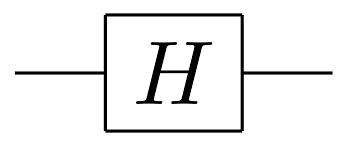
\includegraphics[scale=0.224]{media/bramkaHadamarda.png}
						\end{figure}
					\end{center}
				\end{column}
			\end{columns}					
			\vspace{0.5em}
		\end{block}
	
		\begin{block}{Alternatywna baza}
			\vspace{0.5em}
			$\hat{H}\ket{0}$ oznaczamy przez $\ket{+}$,a $\hat{H}\ket{1}$ przez $\ket{-}$.\\
			$\ket{+}$ i $\ket{-}$ są ortogonalne, więc również wyznaczają bazę.
			\vspace{0.5em}
		\end{block}
	
	\end{frame}
	
	\begin{frame}{Bramki kwantowe}
		\begin{block}{Bramka NOT, $\hat{X}$}
			\vspace{0.5em}
			Bramka neguje stan kwantowy, podobnie jak klasyczny NOT.
			\begin{columns}
				\begin{column}{0.5\textwidth}
					\begin{center}
						$\begin{pmatrix}
						1 & 0\\
						0 & 1 
						\end{pmatrix}$	
					\end{center}	
				\end{column}
				
				\begin{column}{0.5\textwidth}
					\begin{flushleft}
					$\hat{X}\big(\alpha\ket{0}+\beta\ket{1}\big)=\alpha\ket{1}+\beta\ket{0}$
					\end{flushleft}	
				\end{column}
			\end{columns}
			\vspace{0.5em}
			Warto zauważyć że $\hat{X}\hat{X}$ jest macierzą $I$.

				\begin{columns}
					\begin{column}{0.5\textwidth}
						\begin{center}
							
						\end{center}	
					\end{column}
					
					\begin{column}{0.5\textwidth}
						\begin{center}
							\begin{figure}
								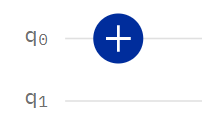
\includegraphics[scale=0.66]{media/bramkaX.png}
							\end{figure}			
						\end{center}	
					\end{column}
				\end{columns}
			\vspace{0.5em}
		\end{block}
	\end{frame}
	
	
	\begin{frame}{Bramki kwantowe}
		\begin{block}{Bramka $\hat{Y}$}
			\vspace{0.5em}
			\begin{columns}
				\begin{column}{0.2\textwidth}
					\begin{flushright}
						$\begin{pmatrix}
						0 & \mbox{-}i\\
						i & 0 
						\end{pmatrix}$	
					\end{flushright}	
				\end{column}
				
				\begin{column}{0.3\textwidth}
					\begin{center}
						\begin{figure}
							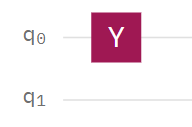
\includegraphics[scale=0.5]{media/bramkaY.png}
						\end{figure}
					\end{center}
				\end{column}
				
				\begin{column}{0.5\textwidth}
					\begin{flushleft}
						$\hat{Y}\big(\alpha\ket{0}\mbox{+}\beta\ket{1}\big)=\mbox{-}i\beta\ket{0}\mbox{+}i\alpha\ket{1}$
					\end{flushleft}	
				\end{column}
			\end{columns}
			\vspace{0.5em}
			$\hat{Y}\hat{Y}$ jest macierzą $I$.
			\vspace{0.5em}
		\end{block}	
	
		\begin{block}{Bramka $\hat{Z}$}
			\vspace{0.5em}
			Bramka zmiany fazy o $\pi$.
			\begin{columns}
				\begin{column}{0.2\textwidth}
					\begin{flushright}
						$\begin{pmatrix}
						1 & 0\\
						0 & \mbox{-}1 
						\end{pmatrix}$	
					\end{flushright}	
				\end{column}
				
				\begin{column}{0.3\textwidth}
					\begin{center}
						\begin{figure}
							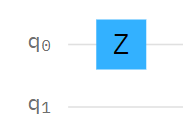
\includegraphics[scale=0.5]{media/bramkaZ.png}
						\end{figure}
					\end{center}
				\end{column}
				
				\begin{column}{0.5\textwidth}
					\begin{flushleft}
						$\hat{Z}\big(\alpha\ket{0}+\beta\ket{1}\big)=\alpha\ket{0}-\beta\ket{1}$
					\end{flushleft}	
				\end{column}
			\end{columns}
			\vspace{0.5em}
			$\hat{Z}\hat{Z}$ jest macierzą $I$.
			\vspace{0.5em}
		\end{block}
	\end{frame}

	\begin{frame}{Stany wielokubitowe}
	
	\begin{block}{}
		\vspace{0.5em}
			Notacja Diraca opisuje też stany wielokubitowe.	
		\vspace{0.5em}
	\end{block}
		\begin{block}{Iloczyn tensorowy}
			\vspace{0.5em}
			Przy jego pomocy można złożyć dwa stany w jeden wypadkowy.\\~\\
			$\ket{\psi_{AB}} = \ket{\psi_{A}}\tens{}\ket{\psi_{B}}=
			\begin{pmatrix}
			\alpha_{A}\\
			\beta_{A}
			\end{pmatrix}$
			$\tens{}\ket{\psi_{B}}=
			\begin{pmatrix}
			\alpha_{A}\ket{\psi_{B}}\\
			\beta_{A}\ket{\psi_{B}}
			\end{pmatrix}
			=
			\begin{pmatrix}
			\alpha_{A}\alpha_{B}\\
			\alpha_{A}\beta_{B}\\
			\beta_{A}\alpha_{B}\\
			\beta_{A}\beta_{B}\\									
			\end{pmatrix}
			$			
			\vspace{0.5em}
		\end{block}
	\end{frame}
		
	\begin{frame}{Układy wielokubitowe}
				\begin{block}{Stany dwukubtitowe}
			\vspace{0.5em}
			Przy pomocy iloczynu tensorowego możemy wyznaczyć  wektory reprezentujące stany własne układu.\\~\\
			\begin{center}
			$
			\ket{00} =
			\begin{pmatrix}
			1\\
			0\\
			0\\
			0
			\end{pmatrix}
			\ket{01} =
			\begin{pmatrix}
			0\\
			1\\
			0\\
			0
			\end{pmatrix}
			\ket{10} =
			\begin{pmatrix}
			0\\
			0\\
			1\\
			0
			\end{pmatrix}
			\ket{11} =
			\begin{pmatrix}
			0\\
			0\\
			0\\
			1
			\end{pmatrix}
			$
			\end{center}
			\vspace{0.5em}
		\end{block}
	\end{frame}
	

	\begin{frame}{Bramki kwantowe}
		\begin{block}{Bramka CNOT}
			\vspace{0.5em}
			Bramka dwukubitowa. Wyróżniamy kubit $control$ i $target$.\\
			$Control$ decyduje o negacji $target$. 
			\begin{columns}
				\begin{column}{0.35\textwidth}
					\begin{center}
						$\begin{pmatrix}
							1 & 0 & 0 & 0\\
							0 & 1 & 0 & 0\\ 
							0 & 0 & 0 & 1\\
							0 & 0 & 1 & 0
						\end{pmatrix}$
					\end{center}	
				\end{column}
				
				\begin{column}{0.35\textwidth}
					\begin{flushleft}
						$\hat{CNOT}\ket{00} = \ket{00}$\\
						$\hat{CNOT}\ket{01} = \ket{01}$\\
						$\hat{CNOT}\ket{10} = \ket{11}$\\
						$\hat{CNOT}\ket{11} = \ket{10}$
					\end{flushleft}	
				\end{column}
			
				\begin{column}{0.3\textwidth}
					\begin{flushright}
						\begin{figure}
						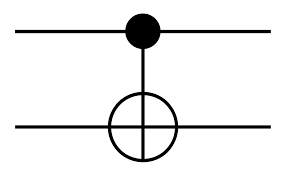
\includegraphics[scale=0.2,left]{media/cnotGate.png}
						\end{figure}		
					\end{flushright}	
				\end{column}
			\end{columns}
			\vspace{0.5em}
		\end{block}
	\end{frame}
	
	\begin{frame}{Splątanie kwantowe}
		
		\begin{block}{Stan splątany$  $}
			\vspace{0.5em}
			\begin{enumerate}
			\item Stanu układu nie da się "rozsupłać".
			\item Zmiana jednego z kubitów wpływa na drugi.
			\item Wystarczy zmierzyć jeden z kubitów, by poznać stan obu.
			\end{enumerate}
			\vspace{0.5em}
		\end{block}	
	\end{frame}

	\begin{frame}{Splątanie kwantowe}
		\begin{block}{Jak splątać kubity?}
			\vspace{0.5em}
			\centering
			Przepuśćmy stan $\ket{00}$ przez poniższy obwód kwantowy.\\~\\
			\centering
			$\ket{00}\xrightarrow{\text{H}}
			\frac{1}{\sqrt{2}}\ket{0}\big(\ket{0}+\ket{1} \big) 
			\xrightarrow{\text{CNOT}}
			\frac{1}{\sqrt{2}}\big(\ket{00} + \ket{11} \big)	
			$
			\vspace{0.8em}
		\end{block}
		\vspace{0.8em}
		\begin{columns}
			\begin{column}{0.5\textwidth}
				\begin{center}
					\begin{figure}[h]
					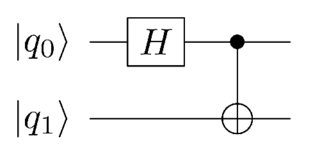
\includegraphics[left]{media/EPR_circuit.jpeg}
					\end{figure}
				\end{center}	
			\end{column}
			
			\begin{column}{0.5\textwidth}
				\begin{center}
				\begin{block}{Wszystkie przypadki "wejścia"}
					\vspace{0.5em}
					$\ket{00}$$\longrightarrow\frac{1}{\sqrt{2}}\big(\ket{00} + \ket{11} \big)$\\
					$\ket{01}$$\longrightarrow\frac{1}{\sqrt{2}}\big(\ket{01} + \ket{10} \big)$\\
					$\ket{10}$$\longrightarrow\frac{1}{\sqrt{2}}\big(\ket{00} - \ket{11} \big)$\\
					$\ket{11}$$\longrightarrow\frac{1}{\sqrt{2}}\big(\ket{01} - \ket{10} \big)$
					\vspace{0.5em}
				\end{block}
				\end{center}	
			\end{column}
		\end{columns}
	
	\end{frame}
	
	\begin{frame}{Splątanie kwantowe}
		
		\begin{block}{Stany Bell'a}
			\vspace{0.5em}
			Tworzą alternatywną bazę dla układów 2 kubitowych.
			\vspace{0.5em}
			\begin{columns}
				\begin{column}{0.5\textwidth}
					\begin{center}
						$\ket{\phi^{+}}=\frac{1}{\sqrt{2}}\big(\ket{00} + \ket{11} \big)$\\	
						$\ket{\psi^{+}}=\frac{1}{\sqrt{2}}\big(\ket{01} + \ket{10} \big)$\\
					\end{center}
				\end{column}
				
				\begin{column}{0.5\textwidth}
					\begin{center}
							$\ket{\phi^{-}}=\frac{1}{\sqrt{2}}\big(\ket{00} - \ket{11} \big)$\\
							$\ket{\psi^{-}}=\frac{1}{\sqrt{2}}\big(\ket{01} - \ket{10} \big)$\\
					\end{center}	
				\end{column}
			\end{columns}
		\end{block}
	
		\begin{block}{Dowód splątania}
			\vspace{0.5em}
			$\ket{\phi^{+}}=\frac{1}{\sqrt{2}}\big(\ket{00} + \ket{11} \big)=\big(\alpha\ket{0}+\beta\ket{1}\big)
			\big(\gamma\ket{0}+\delta\ket{1}\big)=
		 	$ \centering $\alpha\gamma\ket{00}+\alpha\delta\ket{01}+\beta\gamma\ket{10}+\beta\delta\ket{11}$\\~\\
		 	Aby zachodziła równość, $\alpha\gamma=\beta\delta=\frac{1}{\sqrt{2}}$,a  $\alpha\delta=\beta\gamma=0$\\
		 	Ten warunek jest nie do spełnienia.\\Analogicznie dla reszty przypadków.
			\vspace{0.5em}
		\end{block}	
	\end{frame}
	
	\begin{frame}{Protokoły kwantowe - gęste kodowanie}
		\begin{block}{Cel procedury}
			\vspace{0.5em}
			Zakodowanie dwu-bitowej informacji w jednym kubicie. 
			\vspace{0.5em}
		\end{block}
		\begin{block}{Procedura}
			\vspace{0.5em}
				\begin{enumerate}
					\item Przygotowanie splątanego układu
					\item Kodowanie w A
					\item Przesył kubitu z A do B
					\item Dekodowanie w B
				\end{enumerate}
			\vspace{0.5em}
		\end{block}
		
	\end{frame}
	
	\begin{frame}{Protokoły kwantowe - gęste kodowanie}
	
	\only<1>{
	\begin{block}{Krok nr 1}	
		\vspace{0.5em}
		Splątanie kubitów $\ket{0_{\scaleto{A\mathstrut}{4pt}}}$ i $\ket{0_{\scaleto{B\mathstrut}{4pt}}}$w laboratorium i przekazanie ich do punktów A i B.
		\begin{figure}[h]
			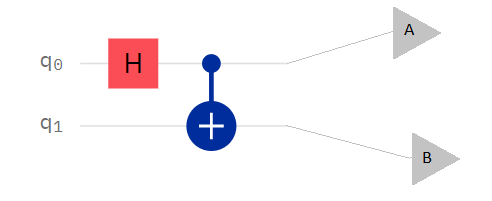
\includegraphics[scale=0.55]{media/entangeling.png}
		\end{figure}
		\vspace{0.5em}
	\end{block}
	}

	\only<2>{
		\begin{block}{Krok nr 2}
			\vspace{0.5em}
			W punkcie A wykonujemy jedną z 4 operacji. Które kodujemy klasycznie.
			
			
			
			\begin{table}[h!]
				\begin{center}
					\begin{tabular}{c|c|c}
						\textbf{Informacja} & \textbf{Operacja} & \textbf{Stan układu}\\
						\hline
						00 & $\hat{I}$ & $\frac{1}{\sqrt{2}}\big(\ket{00}+\ket{11}\big)$\\
						01 & $\hat{X}$ & $\frac{1}{\sqrt{2}}\big(\ket{10}+\ket{01}\big)$\\
						10 & $\hat{Z}$ & $\frac{1}{\sqrt{2}}\big(\ket{00}-\ket{11}\big)$\\
						11 & $\hat{X}\hat{Z}$ & $\frac{1}{\sqrt{2}}\big(\ket{01}-\ket{10}\big)$\\
					\end{tabular}
				\end{center}
			\end{table}	
			\vspace{0.5em}
		\end{block}
	}

	\only<3>{
		\begin{block}{Krok nr 3}	
			\vspace{0.5em}
			Przekazanie kubitu z A do B i wykonanie dekodowania obwodem odwrotnym do obwodu splątującego.
			\begin{figure}[h]
				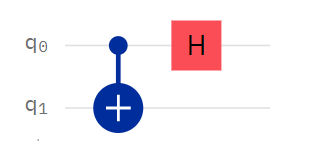
\includegraphics[scale=0.7]{media/reverseEntagler.png}
			\end{figure}
			\vspace{0.5em}
		\end{block}
	}
	
	\only<4>{
		\begin{block}{Krok nr 4}	
			\vspace{0.5em}
			Wykonanie pomiaru na kubitach w punkcie B.\\
			Funkcja opisująca kubit jest postaci $\ket{AB}$, co daje 100\% szansę na odczytanie
			zakodowanej wiadomości.
			\begin{columns}
				\begin{column}{0.66\textwidth}
					\begin{center}
						\begin{figure}
							\centering
							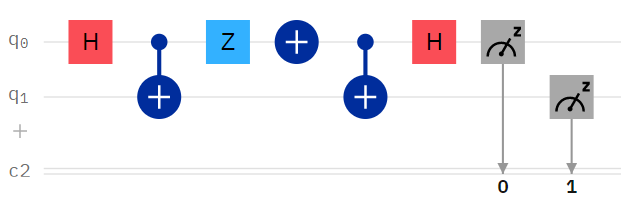
\includegraphics[scale=0.45]{media/denseCodingCircuit.png}
						\end{figure}
					\end{center}	
				\end{column}
				
				\begin{column}{0.34\textwidth}
					\begin{center}
						\begin{figure}
							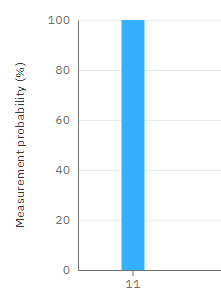
\includegraphics[scale=0.33]{media/denseCodingPropability.png}
						\end{figure}
					\end{center}	
				\end{column}
			\end{columns}
			\vspace{0.5em}
		\end{block}
	}
	\end{frame}
	
	\begin{frame}{Protokoły kwantowe - kwantowa "teleportacja"}
		\only<1>{
		\begin{block}{Cel procedury}
			\vspace{0.5em}
			Transport informacji o kubicie, czyli jego stanu kwantowego, do wskazanego miejsca.
			\vspace{0.5em}
		\end{block}
		\begin{block}{Procedura}
			\vspace{0.5em}
			\begin{enumerate}
			\item Umieszczenie splątanych kubitów w A i B.
			\item Wykonanie pomiaru w bazie Bella, na kubitach z A.
			\item Klasyczny transport informacji o wyniku pomiaru do B.	
			\item Dekodowanie kubitu w B.
		\end{enumerate}
			\vspace{0.5em}
		\end{block}
		}	
		
		\only<2>{
		\begin{block}{Krok 1}
			\vspace{0.5em}
			Splątaną parę kubitów rozdzielamy do punktów A i B.\\W punkcie A znajduje się również kubit $\ket{\psi}$, którego stan przeniesiemy do B.\\~\\
			Stan układu :\\~\\ $\big(\alpha\ket{0}+\beta\ket{1}\big)\frac{1}{\sqrt{2}}\big(\ket{00}+\ket{11}\big)\mbox{=}
			\frac{1}{\sqrt{2}}\big(\alpha\ket{000} + \alpha\ket{011} + \beta\ket{100} + \beta\ket{111}\big)
			$
			
			\vspace{0.5em}
			\begin{figure}[h]
				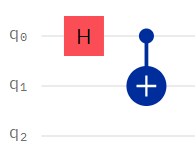
\includegraphics[scale=0.5]{media/teleportationStep1.png}
			\end{figure}
			\vspace{0.5em}
		\end{block}	
		}
	
		\only<3>{
		
		\begin{block}{Krok 2}
			\vspace{0.5em}
			Przedstawmy stan 2 kubitów z A (2 pierwsze) w bazie Bell'a.
			\begin{columns}
				\begin{column}{0.5\textwidth}
					\begin{center}
					$\ket{00} = \ket{\phi^{+}}+\ket{\phi^{-}}$\\
					$\ket{01} = \ket{\psi^{+}}+\ket{\psi^{-}}$\\
					$\ket{10} = \ket{\psi^{+}}-\ket{\psi^{-}}$\\
					$\ket{11} = \ket{\phi^{+}}-\ket{\phi^{-}}$
					\end{center}	
				\end{column}
				
				\begin{column}{0.5\textwidth}
					\begin{center}
						\begin{figure}[h]
							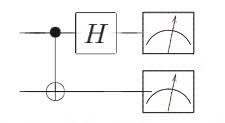
\includegraphics[scale=0.45]{media/bellStateMeasurement.jpeg}
						\end{figure}
					\end{center}	
				\end{column}
			\end{columns}
			\vspace{0.8em}
			Przy pomocy powyższych zależności otrzymujemy:\\
			\vspace{0.8em}
			\centering
			$\big(\frac{1}{\sqrt{2}}\big)^{2}\Big[\ket{\phi^{+}}\big(\alpha\ket{0}+\beta\ket{1}\big)+\ket{\psi^{+}}\big(\alpha\ket{1}+\beta\ket{0}\big)+$\\
			$\ket{\phi^{-}}\big(\alpha\ket{0}-\beta\ket{1}\big)+\ket{\psi^{-}}\big(\alpha\ket{1}-\beta\ket{0}\big)\Big]$
			
			\vspace{0.5em}
		\end{block}
		}
	
		\only<4>{
			
			\begin{block}{Krok 3}
				\vspace{0.5em}
				W zależności o wyniku pomiaru do B zostaje przekazana\\informacja o sposobie przywrócenia informacji o $\ket{\psi}$ na kubicie pozostającym w B.
				\vspace{0.5em}
				\begin{figure}[h]
					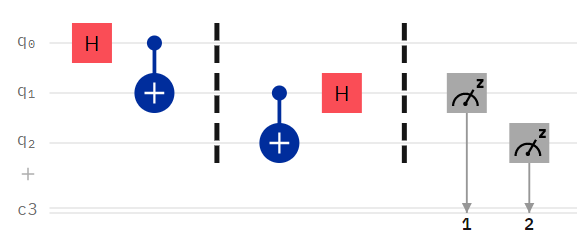
\includegraphics[scale=0.5]{media/teleportationStep3.png}
				\end{figure}
				\vspace{0.5em}
			\end{block}
		}
	
		\only<5>{
			
			\begin{block}{Krok 4}
				\vspace{0.5em} 
				Dzięki informacji z A, wiemy w jakim stanie jest układ po pomiarze.
				Na kubicie z B wykonujemy jedną z operacji :$\hat{I},\hat{X},\hat{Z},\hat{X}\hat{Z}$.
				\vspace{0.5em}
				
				\begin{columns}
					\begin{column}{0.5\textwidth}
					
							\quad Załóżmy, że pomiar w A dał\\ 
							\quad wynik $\ket{\psi^{-}}$. Zachodzi\\
							\quad $collapse$ funkcji falowej\\
							\quad do postaci :$\ket{\psi^{-}}\big(\alpha\ket{1}-\beta\ket{0}\big)$\\
						
					\end{column}
					
					\begin{column}{0.5\textwidth}
						\begin{center}
							\begin{figure}
								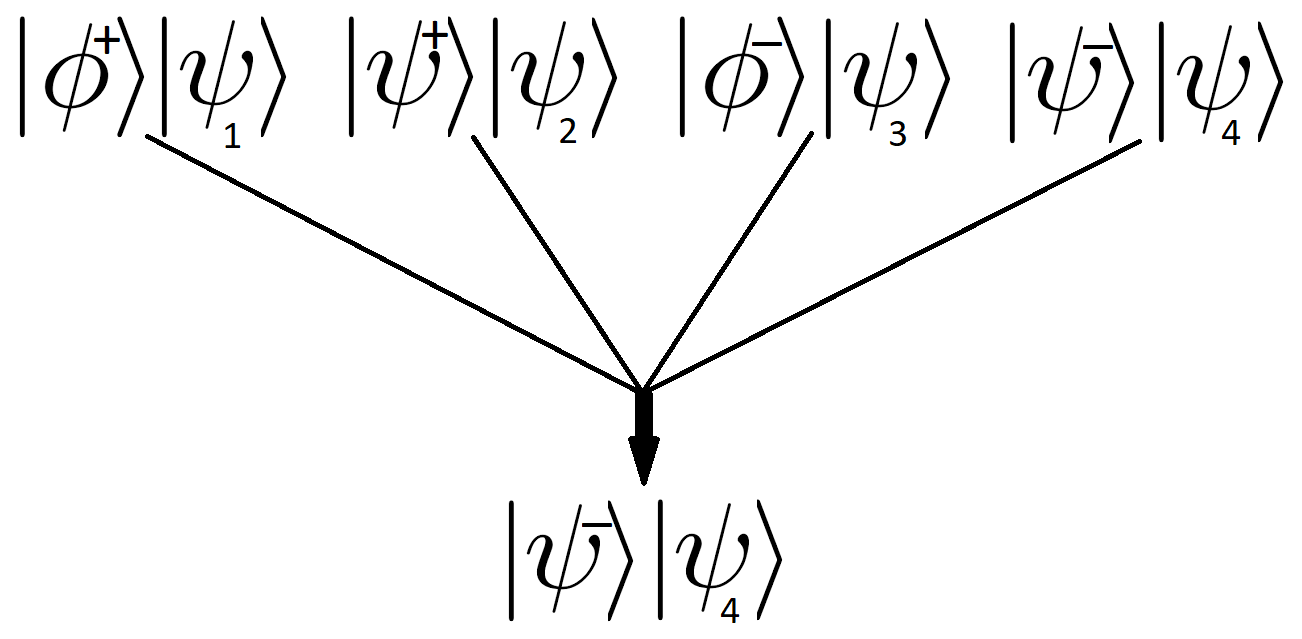
\includegraphics[scale=0.15]{media/collapseExample.png}
							\end{figure}
						\end{center}	
					\end{column}
				\end{columns}
				\vspace{0.5em}
			\end{block}
		}
	
	
		\only<6>{
			
			\begin{block}{Krok 4}
				\vspace{0.5em} 
				Dzięki informacji z A, wiemy w jakim stanie jest układ po pomiarze.
				Na kubicie z B wykonujemy jedną z operacji :$\hat{I},\hat{X},\hat{Z},\hat{X}\hat{Z}$.
				\vspace{0.5em}
				
				Zauważmy, że $\ket{\psi^{-}}\big(\alpha\ket{1}-\beta\ket{0}\big)$ to nic innego jak
				$\hat{Z}\hat{X}\ket{\psi}$.
			\end{block}
						
			\begin{block}{Podsumowanie}
				\vspace{0.5em}
				\begin{columns}
					\begin{column}{0.35\textwidth}

							 \quad Operacja $\hat{X}\hat{Z}$\\ 
							 \quad ustawia stan
							 $\ket{\psi}$, \\
							 \quad tym samym kończąc\\
							 \quad protokół.

					\end{column}
					
					\begin{column}{0.65\textwidth}
						\begin{flushleft}
							\begin{figure}
								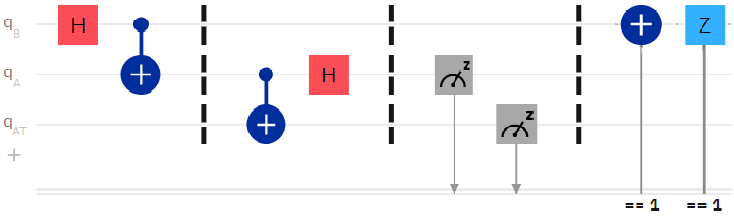
\includegraphics[scale=0.25]{media/QantumTeleportationCircuit.png}
							\end{figure}			
						\end{flushleft}	
					\end{column}
				\end{columns}
				\vspace{0.5em}
			\end{block}
		}
	\end{frame}

	\begin{frame}{Algorytmy kwantowe - Algorytm Groovera}
		\begin{block}{Sformułowanie problemu}
			\vspace{0.5em}
			Istnieje funkcja postaci 
			$\hspace{0.2cm}f:N\rightarrow \{0,1\}$, dana wzorem\\~\\
			\centering
			$
			f(x)=
			\begin{cases}
			0,\hspace{0.2cm} x \neq x_{s}\\
			1,\hspace{0.2cm} x = x_{s}\\
			\end{cases}
			\vspace{0.5em}
			$\\~\\
			Chcemy poznać wartość $x_{s}$.
		\end{block}
	\end{frame}
	
		\begin{frame}{Algorytmy kwantowe - Algorytm Groovera}
		\begin{block}{Podejście klasyczne}
			\vspace{0.5em}
			Iterujemy po wszystkich możliwych wartościach $x$ \\i sprawdzamy czy $f(x_{i})$ jest równe 1.\\~\\
			Złożoność oczywiście : $O(N)$
			\vspace{0.5em}
		\end{block}
		\vspace{0.5em}
		\begin{center}
			\begin{figure}
				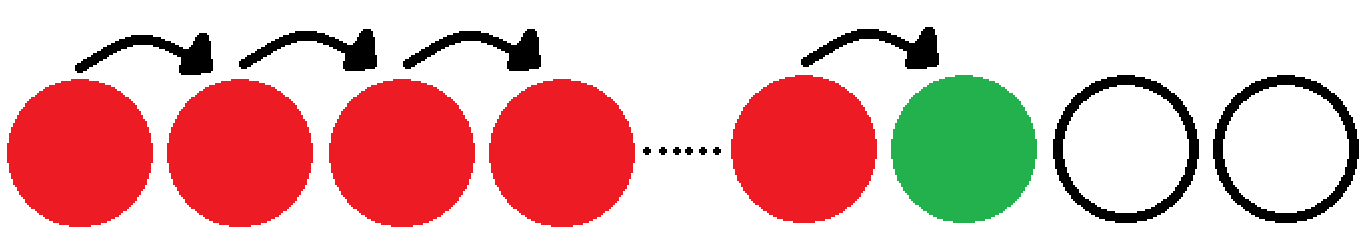
\includegraphics[scale=0.25]{media/classicSearch.png}
			\end{figure}
		\end{center}
	\end{frame}

	\begin{frame}{Algorytmy kwantowe - Algorytm Groovera}
		\begin{block}{Podejście "kwantowe"}
			\vspace{0.5em}
			Algorytm bazuje na iteracyjnym "wzmacnianiu amplitudy" prawdopodobieństwa szukanego stanu $\ket{x_s}$.
			Proces osiągamy poprzez odpowiednie manipulowanie rejestrem kwantowym.
			\vspace{0.5em}
		\end{block}
	\end{frame}

	\begin{frame}{Algorytmy kwantowe - Algorytm Groovera}
		\begin{block}{Krok 1 - Przygotowanie rejestru}

			Niech rejestr kwantowy będzie dany funkcją falową : 
			$$\ket{\phi_{0}} = \frac{1}{\sqrt{N}}\sum\limits_{i=1}^{N-1}\ket{\omega_{i}} $$
			gdzie $N = 2^{n},$ a n to ilość kubitów.\\ \vspace{0.4em}
			Wybieramy taką postać wejściową, ponieważ nie faworyzuje żadnego ze stanów. 
		\end{block}
		\begin{center}
			\begin{figure}
				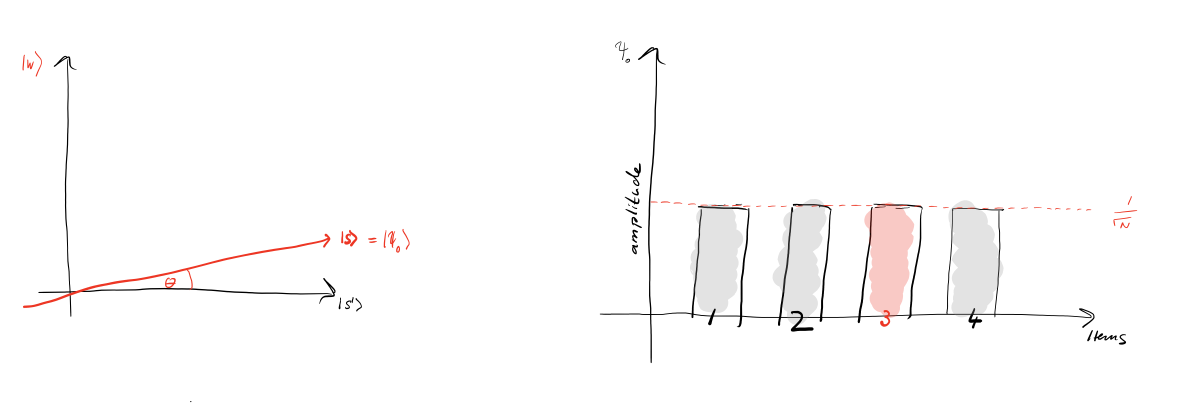
\includegraphics[scale=0.5]{media/groverINIT.png}
			\end{figure}
		\end{center}
	\end{frame}
	
	
	
	\begin{frame}{Algorytmy kwantowe - Algorytm Groovera}
		\begin{block}{Krok 2 - Manipulacje na rejestrze}
			\vspace{0.5em}
			Korzystamy z dwóch operacji (bramek). Nazwijmy je $\mathcal{A}$ i $\mathcal{B}$.\\~\\
			Po każdej iteracji stan rejestru to:
			$$\ket{\phi_{n+1}} =\mathcal{B}\mathcal{A}\ket{\phi_{n}}$$
			\quad gdzie:\\
			\centering
			$\mathcal{A} = \mathcal{I} - 2\ket{\omega_{0}}\bra{\omega_{0}}$\vspace{0.5em}\\
			$\mathcal{B} = 2\ket{\phi_{0}}\bra{\phi_{0}} - \mathcal{I} $\\~\\
			Powtarzamy odpowiednią ilość razy.
			
			\vspace{0.5em}
		\end{block}
	\end{frame}
	
	\begin{frame}{Algorytmy kwantowe - Algorytm Groovera}
		\begin{block}{Operacja $\mathcal{A}$ - "oracle"}
			
			\vspace{0.5em}
			Działanie operatora $\mathcal{A}$ \only<1>{na stan bazowy $\ket{\omega_{i}}$: \\~\\
			$\mathcal{A}\ket{\omega_{i}}= \big(\mathcal{I} - 2\ket{\omega_{0}}\bra{\omega_{0}}\big)\ket{\omega_{i}} =
			 \ket{\omega_{i}} - 2\ket{\omega_{0}}\cdot
			 \begin{cases}
			  0, \quad\omega_{i} \neq\omega_{0}\\
			  1, \quad\omega_{i}= \omega_{0}\\
			 \end{cases}
			$\\
			$
			 \mathcal{A}\ket{\omega_{i}}=
			 \begin{cases}
			 \ket{\omega_{i}},\quad\omega_{i} \neq\omega_{0}\\
			 \mbox{-}\ket{\omega_{i}},\quad\omega_{i}= \omega_{0}\\
			 \end{cases}
			$
			}
			\only<2>{
			na rejestr kwantowy:	
			 
			 \begin{align*}
			 	\mathcal{A}\ket{\phi}&=\mathcal{A}\Big(\sum\limits_{\omega=0}^{N-1}\alpha_{\omega}\ket{\omega}\Big)=
			 	-\alpha_{\omega_{0}}\ket{\omega_{0}}+\sum\limits_{\substack{\omega=0\\\omega\neq\omega_{0}}}^{N-1}\alpha_{\omega}\ket{\omega}
			 \end{align*}
			 
			 
			}
			\vspace{0.5em}
		\end{block}
	
		\begin{center}
			\begin{figure}
				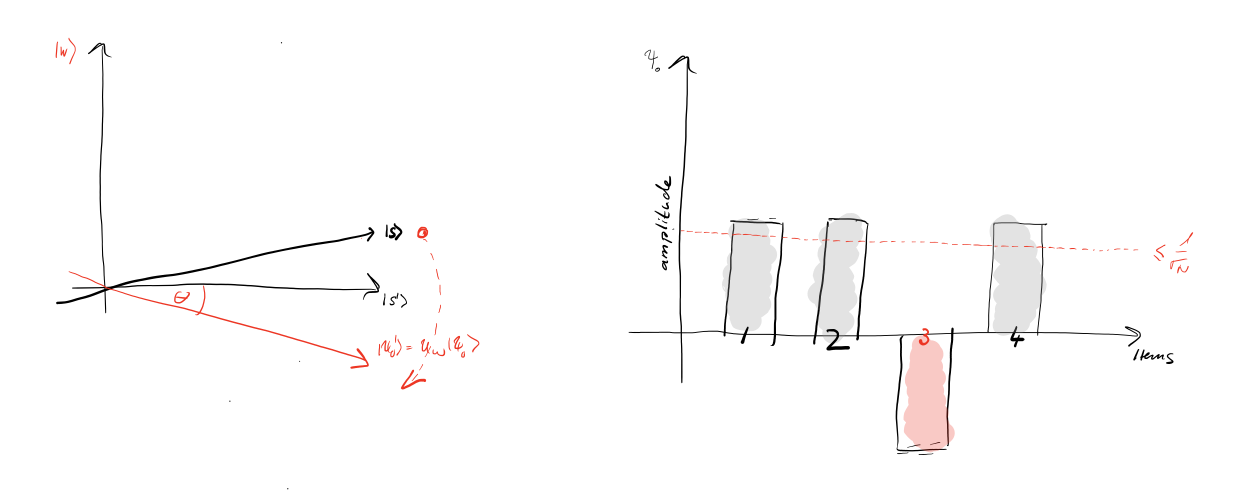
\includegraphics[scale=0.45]{media/grover_A.png}
			\end{figure}
		\end{center}
	\end{frame}
	
	\begin{frame}{Algorytmy kwantowe - Algorytm Groovera}
		\begin{block}{Operacja $\mathcal{B}$}
			\only<1>{\vspace{0.5em}} 
			Działanie operatora $\mathcal{B}$\only<1>{ na stan bazowy $\ket{\omega_{i}}$: \\~\\
				
			$\mathcal{B}\ket{\omega_{i}}= \big(2\ket{\phi_{0}}\bra{\phi_{0}} - \mathcal{I}\big)\ket{\omega_{i}} =
			2\ket{\phi_{0}}\underbrace{\braket{\phi_{0}}{\omega_{i}}}_{=\frac{1}{\sqrt{N}}} - \ket{\omega_{i}}=
			\frac{2}{\sqrt{N}}\ket{\phi_{0}} -\ket{\omega_{i}} $
			\\~\\
			
			$
			\braket{\phi_{0}}{\omega_{i}}=
			\begin{pmatrix}
			\frac{1}{\sqrt{N}} & \frac{1}{\sqrt{N}} & \cdots & \frac{1}{\sqrt{N}} & \frac{1}{\sqrt{N}}
			\end{pmatrix}
			\cdot
			\begin{pmatrix}
			0 & 1 & \cdots & 0 & 0
			\end{pmatrix}
			^{T}
			= \frac{1}{\sqrt{N}}
			$
			}
			\only<2>{
				na rejestr kwantowy:
				\begin{align*}
					\mathcal{B}\ket{\phi} &= \mathcal{B}\big(\sum\limits_{\omega=0}^{N-1}\alpha_{\omega}\ket{\omega}\big)= \sum\limits_{\omega=0}^{N-1}\alpha_{\omega}\big(\frac{2}{\sqrt{N}}\ket{\phi_{0}}-\ket{\omega}\big)\\
					&=\frac{2}{\sqrt{N}}=\sum\limits_{\omega=0}^{N-1}\alpha_{\omega}\Big(\frac{1}{\sqrt{N}}\sum\limits_{\omega=0}^{N-1}\ket{\omega}\Big)-
					\sum\limits_{\omega=0}^{N-1}\alpha_{\omega}\ket{\omega}\\
					&=\underbrace{\frac{2}{N}\sum\limits_{\omega=0}^{N-1}\alpha_{\omega}}_{\alpha_{avg}}\sum\limits_{\omega=0}^{N-1}\ket{\omega}-\sum\limits_{\omega=0}^{N-1}\alpha_{\omega}\ket{\omega}\\
					&=\sum\limits_{\omega=0}^{N-1}\big(2\alpha_{avg}-\alpha_{\omega}\big)\ket{\omega}=\sum\limits_{\omega=0}^{N-1}\Big(\alpha_{avg} + (\alpha_{avg}-\alpha_{\omega})\Big)\ket{\omega}
				\end{align*}
			}
		
		\end{block}
		\only<1>{
		\begin{center}
			\begin{figure}
				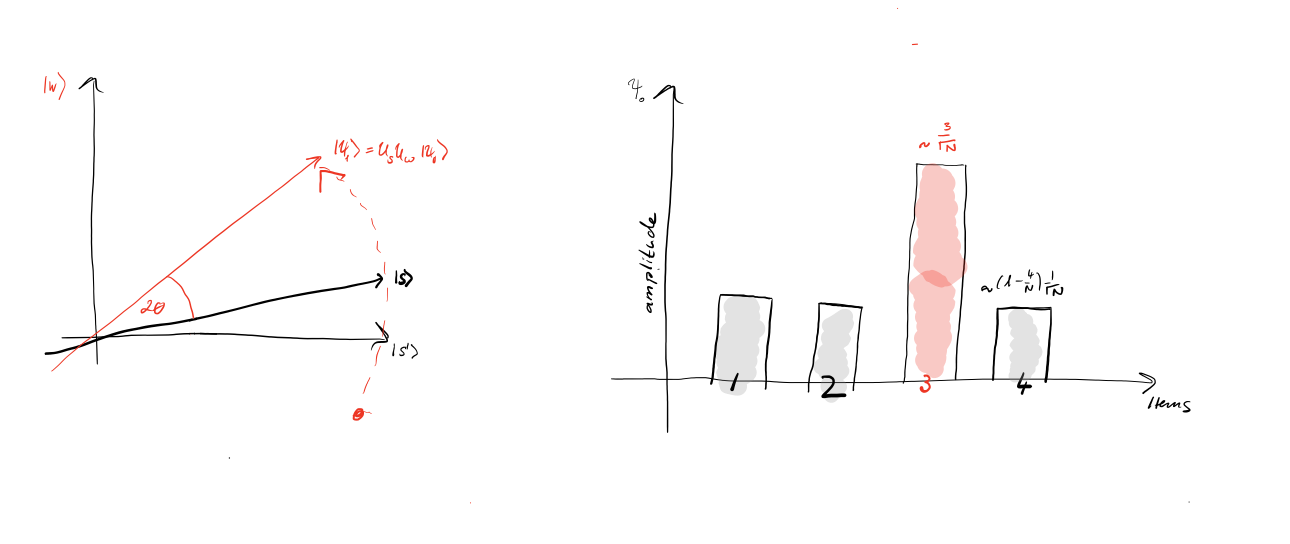
\includegraphics[scale=0.45]{media/grover_B.png}
			\end{figure}
		\end{center}
		}
	\end{frame}
	
	\begin{frame}{Algorytmy kwantowe - Algorytm Groovera}
			\vspace{0.5em}
			\begin{center}
				\begin{figure}
					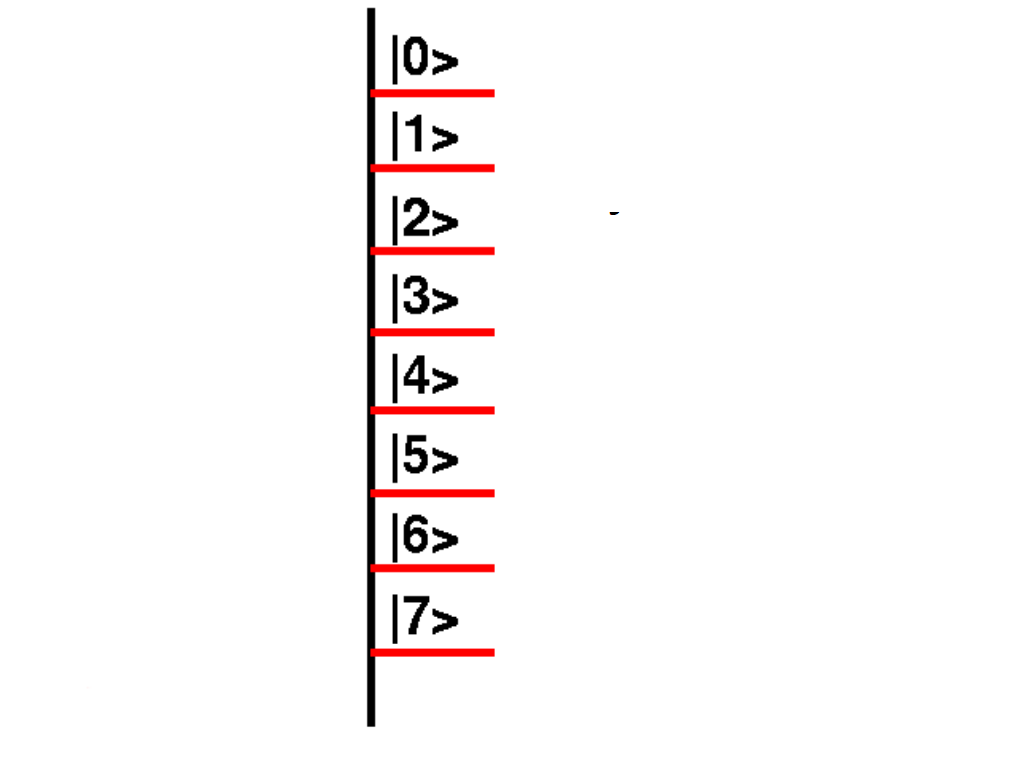
\includegraphics[scale=0.35]{media/visualization1.png}
				\end{figure}
			\end{center}
			\vspace{0.5em}
	\end{frame}
	
	\begin{frame}{Algorytmy kwantowe - Algorytm Groovera}
		\vspace{0.5em}
		\begin{center}
			\begin{figure}
				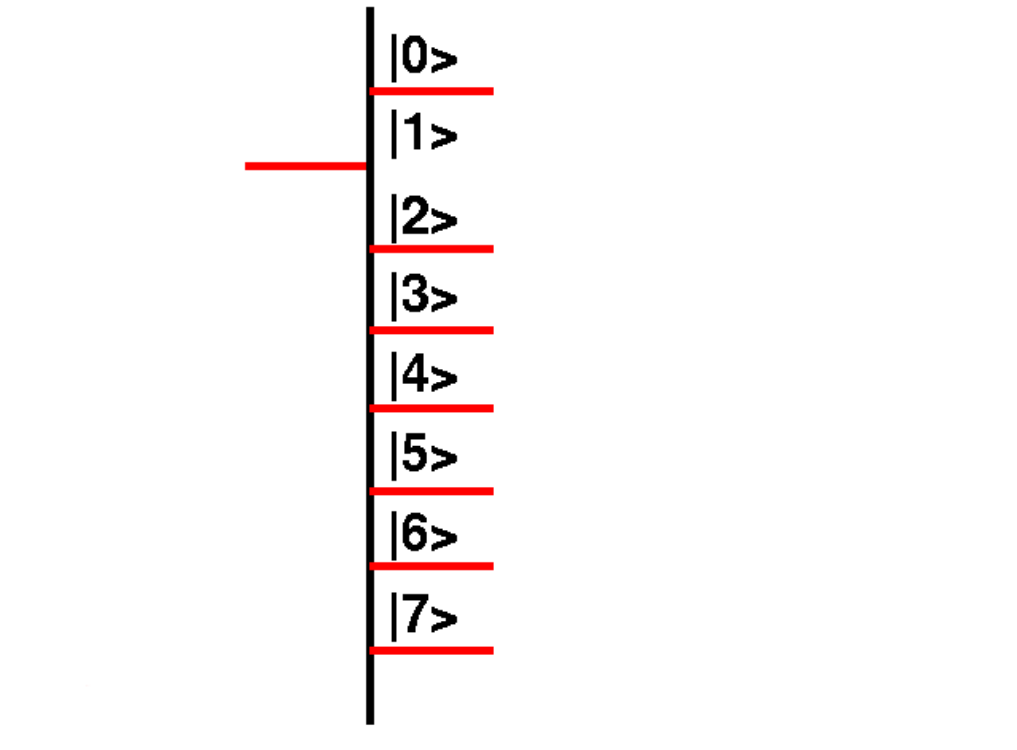
\includegraphics[scale=0.35]{media/visualization2.png}
			\end{figure}
		\end{center}
		\vspace{0.5em}
	\end{frame}
		
	\begin{frame}{Algorytmy kwantowe - Algorytm Groovera}
		\vspace{0.5em}
		\begin{center}
			\begin{figure}
				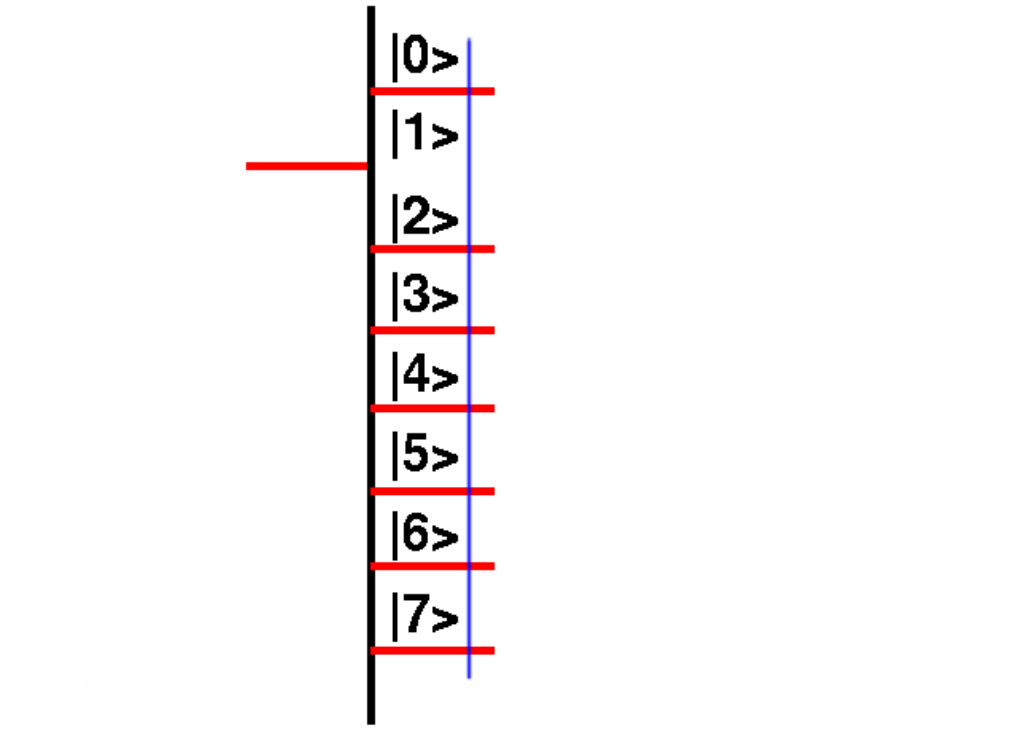
\includegraphics[scale=0.35]{media/visualization3.png}
			\end{figure}
		\end{center}
		\vspace{0.5em}
	\end{frame}		
	
		\begin{frame}{Algorytmy kwantowe - Algorytm Groovera}
		\vspace{0.5em}
		\begin{center}
			\begin{figure}
				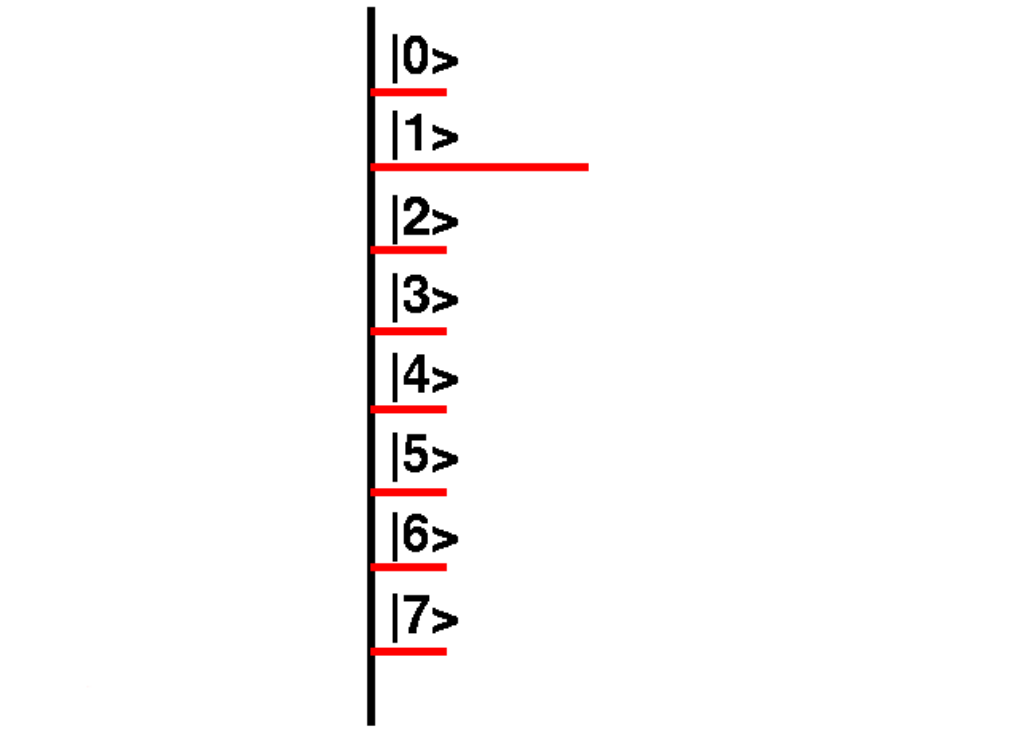
\includegraphics[scale=0.35]{media/visualization4.png}
			\end{figure}
		\end{center}
		\vspace{0.5em}
	\end{frame}
	
	\begin{frame}{Algorytmy kwantowe - Algorytm Groovera}
		\vspace{0.5em}
		\begin{center}
			\begin{figure}
				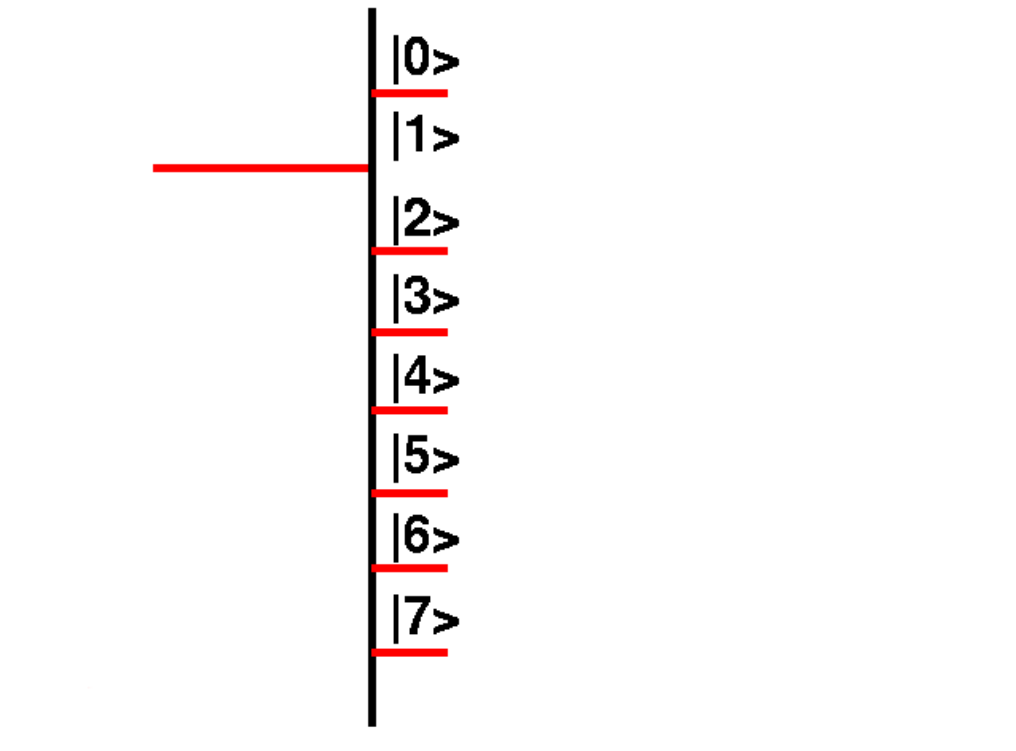
\includegraphics[scale=0.35]{media/visualization5.png}
			\end{figure}
		\end{center}
		\vspace{0.5em}
	\end{frame}
	
	\begin{frame}{Algorytmy kwantowe - Algorytm Groovera}
		\vspace{0.5em}
		\begin{center}
			\begin{figure}
				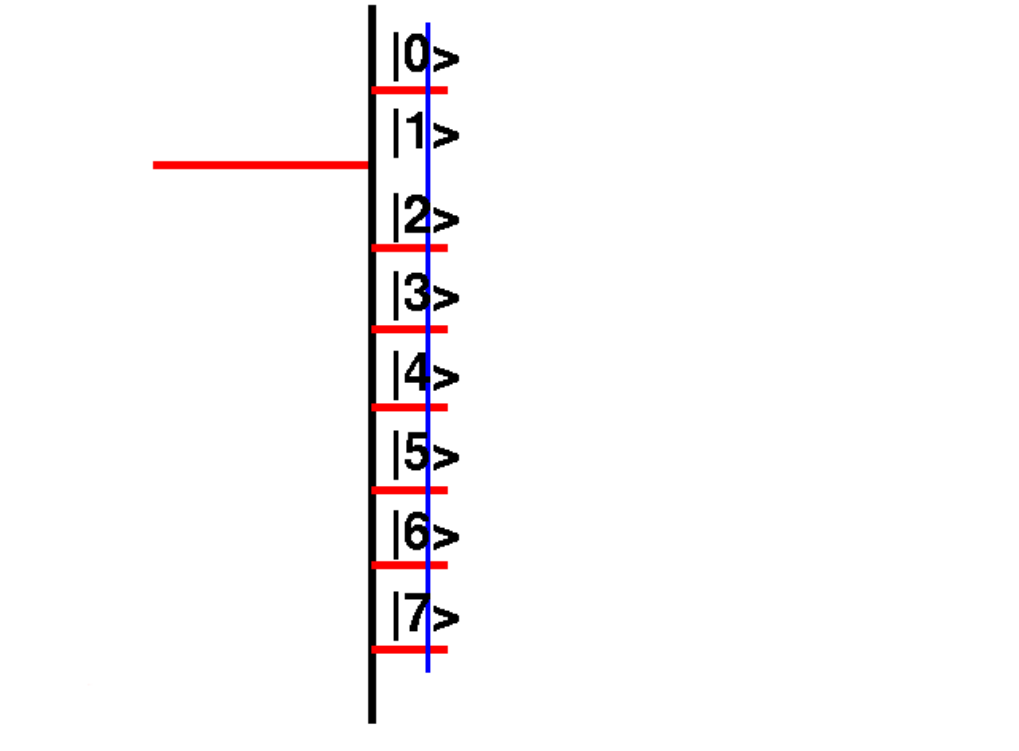
\includegraphics[scale=0.28]{media/visualization6.png}
			\end{figure}
		\end{center}
		\vspace{0.5em}
	\end{frame}	
	
	
	\begin{frame}{Algorytmy kwantowe - Algorytm Groovera}
		\vspace{0.5em}
		\begin{center}
			\begin{figure}
				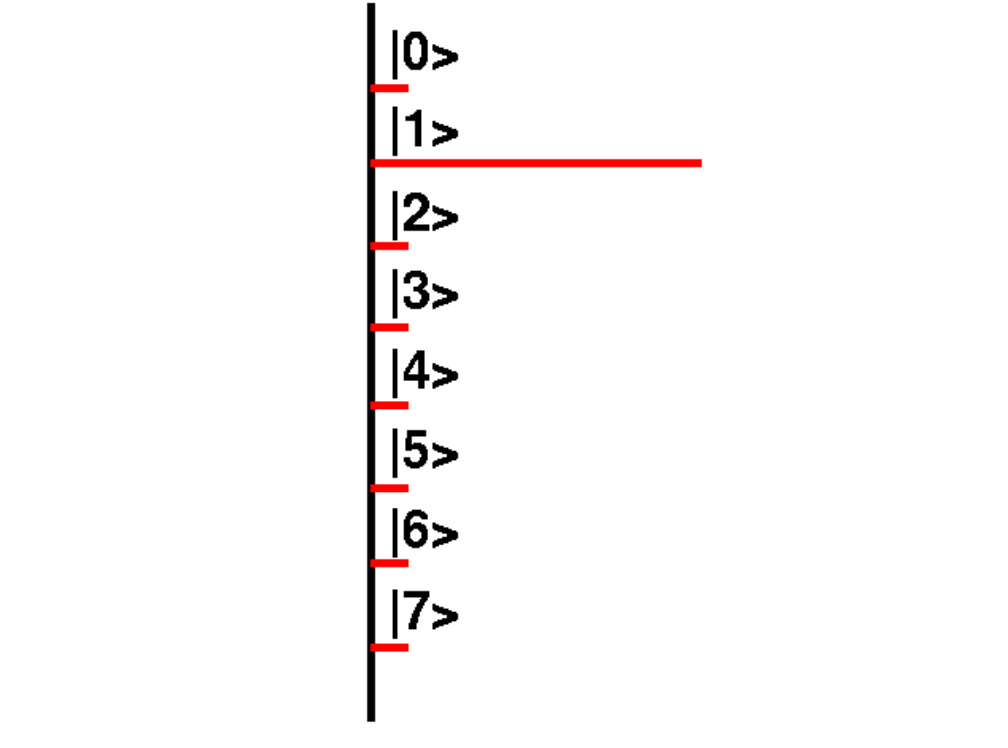
\includegraphics[scale=0.28]{media/visualization7.png}
			\end{figure}
		\end{center}
		\vspace{0.5em}
	\end{frame}	
		
	\begin{frame}{Algorytmy kwantowe - Algorytm Groovera}
		\vspace{0.5em}

	
		\begin{block}{Podsumowanie i implementacja}
			\vspace{0.5em}
			
			Ilość operacji $\mathcal{B}\mathcal{A}$ to: $\floor{\frac{\pi}{4}\sqrt{N} - \frac{1}{2}}\implies O(\sqrt{N})$ \\~\\
			Po wykonanych operacjach algorytm kończy się pomiarem.\\~\\
			Prawdopodobieństwo sukcesu $P(\checkmark) \approx 1 - \frac{1}{N} $
			\begin{center}
				\begin{figure}
					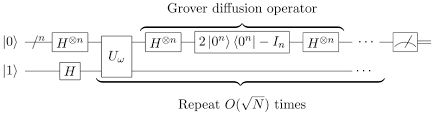
\includegraphics[scale=0.55]{media/groverCircuit.png}
				\end{figure}
			\end{center}
		\vspace{1em}	
		\end{block}
	\end{frame}

	\begin{frame}{Praktyczne zastosowanie}
		
	\end{frame}
	
	\begin{frame}{Praktyczne zastosowanie}
		
	\end{frame}
	
	
	
	
	
	\begin{frame}{Bibliografia}
		\begin{block}{}
			\vspace{0.5em}
			\begin{enumerate}
			\item skrypt "kubity.pdf", dr inż. Tomasz Gradowski 
			\item \href{https://www.youtube.com/watch?v=puRu_wEsbAA}{nagrania YT "Wszechnica CFT PAN: Części 1-12",\\ mgr K. Kowalczyk-Murynka}
			\item Wikipedia 
			\item \href{https://robert.nowotniak.com/files/papers/grover.pdf}{"Algorytm Grovera"}, Dr Robert Nowotniak
			\end{enumerate}
			\vspace{0.5em}
		\end{block}	
	\end{frame}

	\begin{frame}{Koniec}
		\begin{block}{}
			\vspace{0.5em}
			\begin{center}
				Dziękuję za uwagę.\\
				Proszę o {\huge proste} pytania.
			\end{center}
			\vspace{0.5em}
		\end{block}
	\end{frame}
	


\end{document}  